\documentclass[border=10pt]{standalone}
\usepackage{tikz}\usepackage{amsmath}\usetikzlibrary{arrows.meta}
\begin{document}
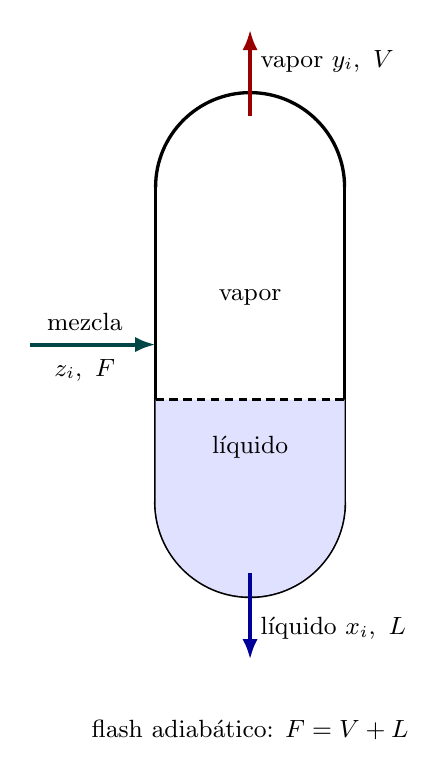
\begin{tikzpicture}[line width=1pt,>={Latex[length=2.6mm]}]
  % recipiente vertical
  \draw[line width=1.2pt] (0,0) -- (0,4) (2.4,0) -- (2.4,4);
  \draw[line width=1.2pt] (0,4) arc (180:0:1.2);
  \draw[line width=1.2pt] (0,0) arc (180:360:1.2);
  % liquido abajo
  \fill[blue!12] (0,0) arc (180:360:1.2) -- (2.4,1.3) -- (0,1.3) -- cycle;
  \draw[densely dashed] (0,1.3)--(2.4,1.3);
  \node at (1.2,0.7){\small líquido};
  \node at (1.2,2.6){\small vapor};
  % alimentacion (entra al lado)
  \draw[->,teal!55!black,line width=1.4pt] (-1.6,2.0)--(0,2.0);
  \node[above] at (-0.9,2.05){\small mezcla};
  \node[below] at (-0.9,1.95){\small $z_i,\ F$};
  % vapor sale arriba
  \draw[->,red!60!black,line width=1.4pt] (1.2,4.9)--(1.2,6.0);
  \node[right] at (1.2,5.6){\small vapor $y_i,\ V$};
  % liquido sale abajo
  \draw[->,blue!60!black,line width=1.4pt] (1.2,-0.9)--(1.2,-2.0);
  \node[right] at (1.2,-1.6){\small líquido $x_i,\ L$};
  \node at (1.2,-2.9){\small flash adiabático: $F=V+L$};
\end{tikzpicture}
\end{document}
